\documentclass[border=10pt]{standalone}

\usepackage{tikz}
\usepackage{tikzsymbols}
\usetikzlibrary{calc,patterns,shapes.geometric}

\def\centerarc[#1](#2)(#3:#4:#5){\draw[#1] ($(#2)+({#5*cos(#3)},{#5*sin(#3)})$) arc (#3:#4:#5);}

\begin{document}
	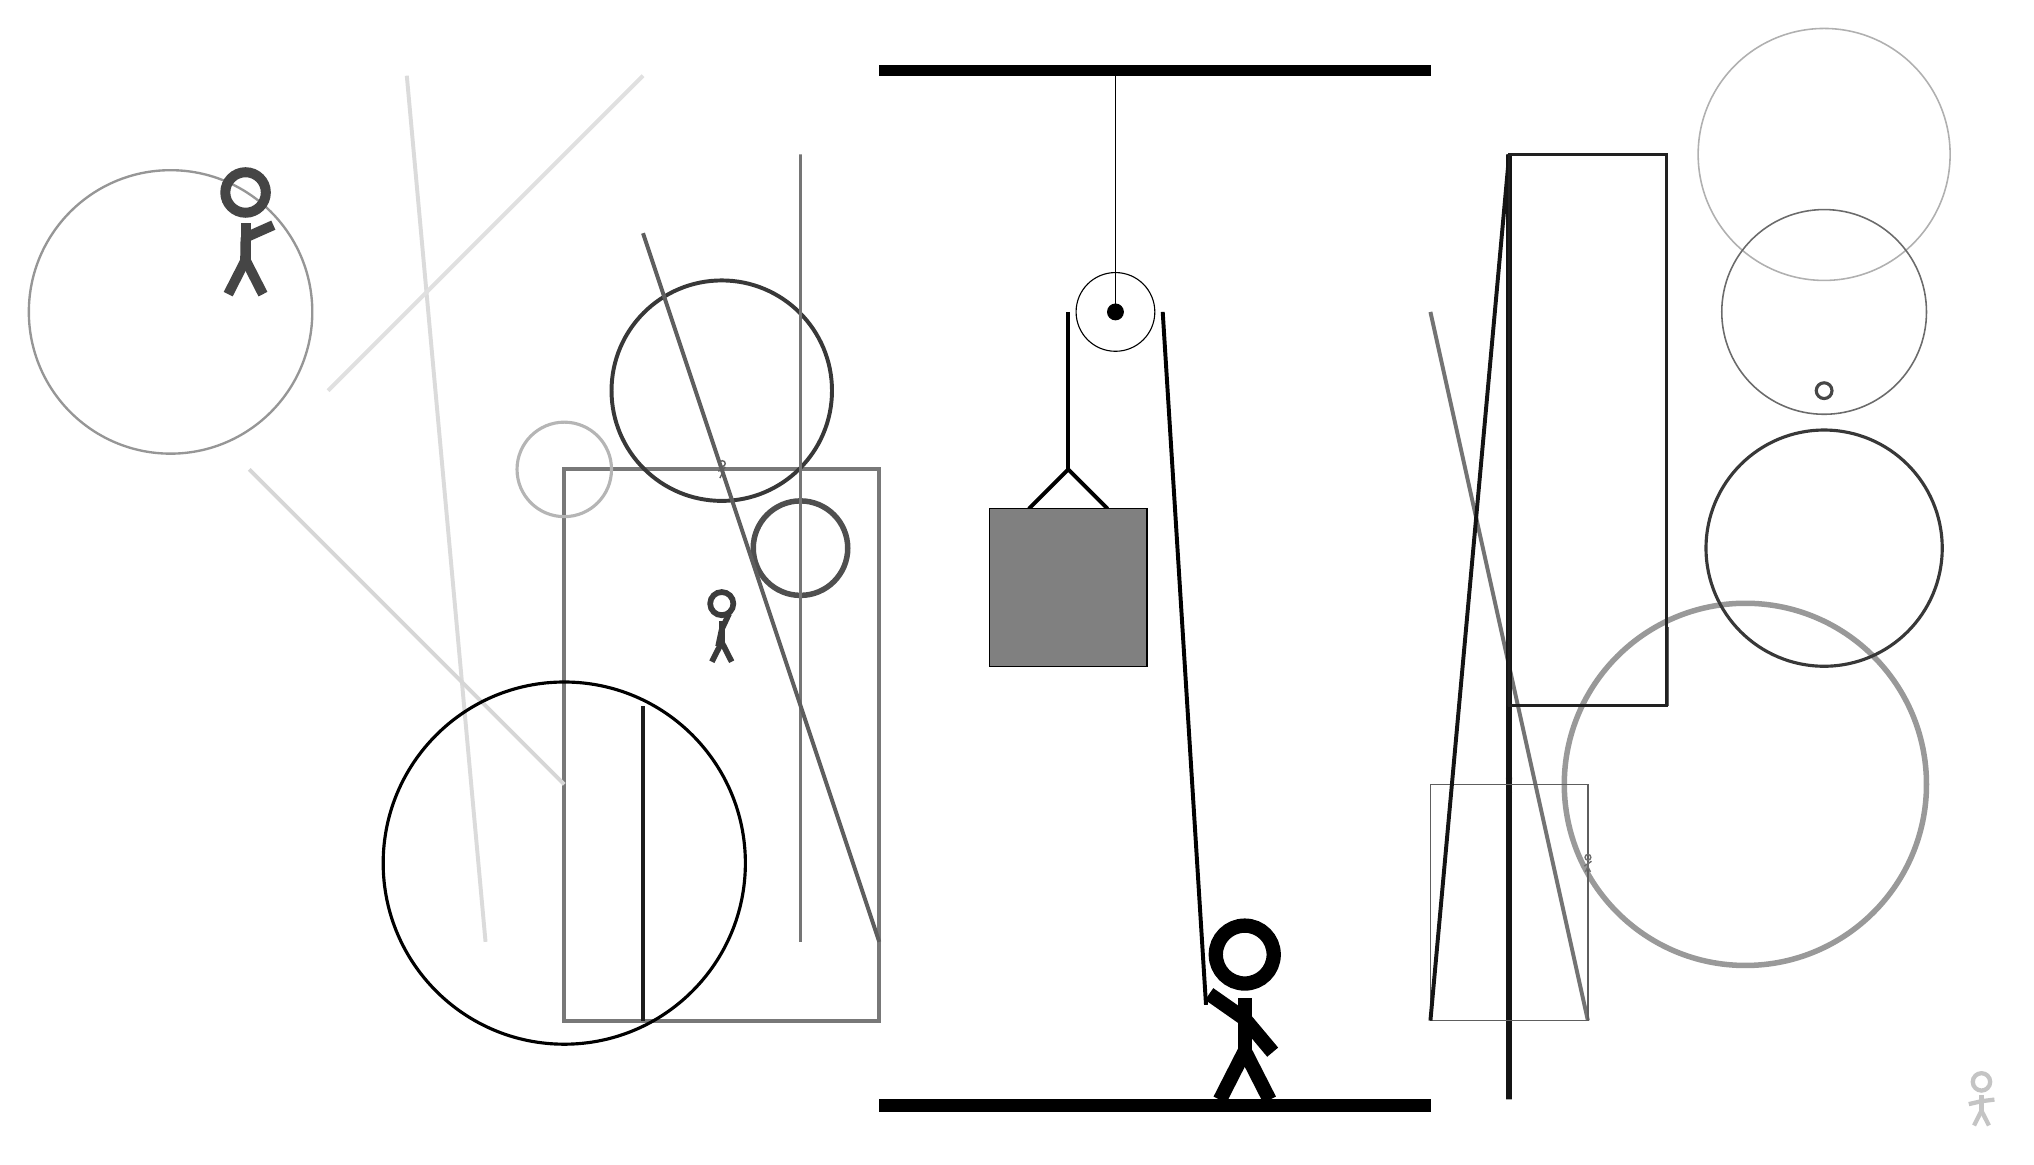
\begin{tikzpicture}
		%%%%% START %%%%%
		
		\draw[fill=black] (-2, 10) rectangle (5, 10.125);
		
		\draw (1, 7) circle (0.5);
		\draw[fill=black] (1, 7) circle (0.1);
		\draw (1, 10) -- (1, 7);
		
		\draw [line width=0.4mm, color=black!72](10, 6) circle (0.1);
		
		\draw [line width=0.2mm, color=black!31](10, 9) circle (1.6);
		\draw[line width=0.5mm, color=black!53] (-2, -2) rectangle (-6, 5);
		\draw[line width=0.5mm, color=black!14](-7, -1) -- (-8, 10);
		\draw[line width=0.5mm, color=black!16](-6, 1) -- (-10, 5);
		
		\draw[line width=0.5mm, color=black!55](7, -2) -- (5, 7);
		
		\draw [line width=0.5mm, color=black!78](-4, 6) circle (1.4);
		\draw [line width=0.7mm, color=black!69](-3, 4) circle (0.6);
		\draw [line width=0.3mm, color=black!41](-11, 7) circle (1.8);
		\draw[line width=0.4mm, color=black!54] (-3, -1) rectangle (-3, 9);
		
		\draw [line width=0.4mm, color=black!100](-6, 0) circle (2.3);
		\draw [line width=0.7mm, color=black!40](9, 1) circle (2.3);
		\draw[line width=0.5mm, color=black!61](8, 3) -- (8, 2);
		
		\node[line width=0.7mm, color=black!62] at (-4, 5) {\Strichmaxerl[1][13][45]};
		\node[line width=0.4mm, color=black!11] at (6, 1) {\Strichmaxerl[1][57][83]};
		\draw[line width=0.7mm, color=black!92] (6, -3) rectangle (6, 9);
		
		\draw[line width=0.5mm, color=black!89](-5, -2) -- (-5, 2);
		\draw[line width=0.2mm, color=black!63] (7, 1) rectangle (5, -2);
		\draw[line width=0.5mm, color=black!90](6, 5) -- (6, 2);
		\draw[line width=0.5mm, color=black!63](-2, -1) -- (-5, 8);
		\draw[line width=0.5mm, color=black!12](-5, 10) -- (-9, 6);
		\node[line width=0.2mm, color=black!77] at (-4, 3) {\Strichmaxerl[4][78][65]};
		
		\draw[line width=0.5mm, color=black!92](6, 9) -- (5, -2);
		\node[line width=0.5mm, color=black!57] at (7, 0) {\Strichmaxerl[1][33][35]};
		\node[line width=0.2mm, color=black!23] at (12, -3) {\Strichmaxerl[3][13][7]};
		
		\draw[line width=0.3mm, color=black!87] (6, 2) rectangle (8, 9);
		
		\draw [line width=0.4mm, color=black!29](-6, 5) circle (0.6);
		\draw [line width=0.4mm, color=black!78](10, 4) circle (1.5);
		\draw [line width=0.2mm, color=black!58](10, 7) circle (1.3);
		
		\node[line width=0.7mm, color=black!73] at (-10, 8) {\Strichmaxerl[7][89][24]};
		
		\draw[line width=0.5mm] (-0.1, 4.5) -- (0.4, 5.0) -- (0.9, 4.5);
		\draw[fill=black!50] (-0.6, 4.5) rectangle (1.4, 2.5);
		
		\draw[line width=0.5mm] (0.4, 7) -- (0.4, 5.0);
		\centerarc[line width=0.5mm](1, 7)(0:180:0.6);
		\draw[line width=0.5mm](1.6, 7) -- (2.15, -1.8);
		
		\node at (2.6, -1.9) {\Strichmaxerl[10][-35][-50]};
		
		\draw[fill=black] (-2, -3) rectangle (5, -3.15);
		
		%%%%% END %%%%%
	\end{tikzpicture}
\end{document}